\documentclass[conference]{IEEEtran}
\IEEEoverridecommandlockouts

\usepackage{cite}
\usepackage{amsmath,amssymb,amsfonts}
\usepackage{algorithmic}
\usepackage{graphicx}
\usepackage{textcomp}
\usepackage{xcolor}
\usepackage{booktabs}
\usepackage{url}
\def\BibTeX{{\rm B\kern-.05em{\sc i\kern-.025em b}\kern-.08em T\kern-.1667em\lower.7ex\hbox{E}\kern-.125emX}}

\begin{document}

\title{Operationalizing Verification and Validation for Text Corpora:\\
A Parameter-Free Information-Theoretic Framework}

\author{
\IEEEauthorblockN{Emmanuel Okoaze\IEEEauthorrefmark{1},
William J. Teahan\IEEEauthorrefmark{1}}
\IEEEauthorblockA{\IEEEauthorrefmark{1}
School of Computer Science\\
Bangor University\\
Bangor, United Kingdom\\
mmk25kng@bangor.ac.uk, w.teahan@bangor.ac.uk
}
}

\maketitle

\begin{abstract}
Corpora underpin empirical work in computational linguistics, yet the corpus
itself is rarely subjected to the systematic verification and validation (V\&V)
that comparable engineering disciplines require. We present a framework that
makes corpus V\&V operational and measurable. First, we recast the
verification/validation distinction as a falsifiable prediction about which
measurement instrument detects which class of defect, rather than as a
descriptive taxonomy. Second, we introduce Reciprocal Good--Turing (RGT)
smoothing, a parameter-free estimator for divergence between two corpora: the
reserved probability mass is set by the Good--Turing singleton estimate and
redistributed over unseen n-grams in proportion to the comparison partner's
distribution. RGT eliminates the free smoothing parameter, self-adapts across
n-gram orders by two orders of magnitude on the same texts, and yields a
conservative divergence estimate. Third, we evaluate detection against controlled
ground truth: five defect classes injected at known rates into clean corpora,
giving 2{,}400 corpus-level and 360 document-level measurements. RGT is monotonic
in defect rate for every defect class and attains larger effect sizes than
add-$k$ smoothing at every setting of $k$ examined for encoding corruption
($d=1.93$ versus a range of $0.47$--$1.58$), while requiring no parameter choice.
A frequency-profile measure representative of established practice is
non-monotonic on encoding corruption and exhibits a \emph{negative} effect size
($d=-0.80$, $p=1.000$), reporting a more corrupted corpus as more similar to its
clean reference. The framework's central prediction is confirmed: content defects
are detected at the corpus level with effect sizes at least $6.5\times$ those of
structural defects, none of which survives correction for multiple comparisons,
whereas structural defects are detected perfectly at the document level (ROC-AUC
$=1.000\pm0.000$).
\end{abstract}

\begin{IEEEkeywords}
corpus quality, verification and validation, Jensen--Shannon divergence,
Good--Turing estimation, smoothing, defect injection, language resources
\end{IEEEkeywords}

\section{Introduction}

Empirical computational linguistics rests on corpora, but the corpus is seldom
treated as an engineered artifact whose fitness for purpose must be
demonstrated. Kilgarriff's observation that corpus linguistics harbours a
methodological void at its centre \cite{kilgarriff2001} remains apposite: the
object at the heart of the research is the object least often subjected to
quality control.

Recent large-scale audits have made the cost of this omission concrete. A manual
audit of 205 language-specific corpora drawn from five major public multilingual
datasets found that at least fifteen contained no usable text at all, that a
substantial fraction consisted of less than half acceptable-quality sentences,
and that scores of corpora were mislabelled or carried nonstandard language
codes \cite{kreutzer2022}. Duplication in training corpora has separately been
shown to degrade downstream language models \cite{lee2022dedup}. These are not
exotic failures; they are precisely the defects a routine quality-management
process would catch.

Software and systems engineering formalize such a process as \emph{verification
and validation} \cite{boehm1984,ieee1012}. Verification asks whether the artifact
was built correctly against its specification; validation asks whether the right
artifact was built for the user's needs. Applied to corpora, verification
concerns structure:empty or truncated documents, duplicates, inconsistent
markup, mismatched document counts across a parallel pair---while validation
concerns content: whether the text is in the language claimed, whether it is
representative, whether annotations are correct.

Making this operational requires answering two questions that the literature
leaves open. \emph{Which instrument detects which defect?} A taxonomy that
classifies defects but does not tell a practitioner what to measure is of limited
use. \emph{And how do we know a proposed measure detects anything?} A measure is
commonly demonstrated by computing it between two well-known corpora, obtaining a
small number, computing it between two dissimilar corpora, obtaining a larger
number, and observing that the ordering is intuitive. This establishes that the
measure ranks obviously-different texts above obviously-similar ones. It does not
establish detection, because no defect was present to detect and no correct
answer was available for comparison.

We address both questions. For the second we construct ground truth by
\emph{controlled defect injection}: starting from clean corpora, we inject
defects of known type at known rates, so the correct answer is known by
construction. This supports dose--response curves, effect sizes, significance
tests, and comparison against a baseline---the standard apparatus for validating
a detection method.

Our contributions are:

\begin{enumerate}
  \item \textbf{An operational V\&V framework} that maps each defect class to the
        instrument that detects it, stated as a falsifiable prediction and
        confirmed experimentally (Sections~\ref{sec:framework}
        and~\ref{sec:results}).
  \item \textbf{Reciprocal Good--Turing smoothing}, a parameter-free estimator
        for corpus divergence that derives its smoothing mass from the data and
        redistributes it using the comparison partner rather than uniformly
        /*(Section~\ref{sec:rgt})*/. It removes a free parameter whose choice we show
        can change measured effect size more than threefold.
  \item \textbf{A controlled defect-injection benchmark} for corpus V\&V,
        comprising 2{,}400 corpus-level and 360 document-level measurements over
        five defect classes and eight injection rates
        (Sections~\ref{sec:design}--\ref{sec:results}).
\end{enumerate}

\section{Related Work}

\subsection{Corpus comparison measures}
Kilgarriff and Rose surveyed measures for corpus similarity and homogeneity,
recommending a $\chi^2$ statistic computed over word-frequency profiles
\cite{kilgarriff1998,kilgarriff2001}. Frequency-profile comparison remains the
established informal instrument for judging whether two corpora resemble one
another, and we adopt a normalized form of it as our baseline for exactly that
reason.

\subsection{Compression, entropy, and divergence}
Compression provides a practical estimator of cross-entropy, and PPM-family
models have been used to estimate the entropy of natural language
\cite{cleary1984,teahan1996}. The connection to divergence is direct: the excess
codelength incurred when coding one corpus with a model trained on another is the
Kullback--Leibler divergence between them \cite{cover2006}. The Jensen--Shannon
divergence \cite{lin1991} provides a symmetric, bounded alternative whose square
root satisfies the triangle inequality \cite{endres2003}.

\subsection{Smoothing}
Estimating a divergence requires nonzero probabilities across the union of two
vocabularies, which makes smoothing unavoidable. Add-$k$ (Lidstone) and related
schemes are surveyed in \cite{chen1999}. Good--Turing estimation
\cite{good1953,gale1995} instead derives the mass reserved for unseen events from
the frequency-of-frequencies of the observed sample. In information retrieval,
document language models are commonly smoothed toward a background collection
model \cite{zhai2004}. Our estimator (Section~\ref{sec:rgt}) combines the
Good--Turing mass estimate with a redistribution conditioned on the comparison
partner; we state the relationship to this prior work precisely in
Section~\ref{sec:rgt-novelty}.

\subsection{Corpus documentation and auditing}
Datasheets \cite{gebru2021} and data statements \cite{bender2018} standardize
what should be \emph{recorded} about a dataset; audits of C4 \cite{dodge2021} and
of web-crawled multilingual corpora \cite{kreutzer2022} report what is actually
\emph{found} in them. These are complementary to our concern: they prescribe
documentation and report manual findings, whereas we ask which automatic
measurement reliably detects a given defect and demonstrate it against ground
truth.

\section{An Operational V\&V Framework}
\label{sec:framework}

We take verification to concern the \emph{structure} of a corpus and validation
to concern its \emph{content}. The substantive claim is that this is not
bookkeeping but a statement about where the evidence for a defect resides.

A structural defect perturbs the arrangement of documents while leaving the
aggregate distribution of linguistic material largely intact. Replacing one
document with a copy of another changes no token's corpus-wide frequency by more
than a small amount; truncating a few documents removes tokens roughly in
proportion to their existing frequencies. The aggregate n-gram distribution
barely moves, and the evidence lives in relations \emph{between} documents.

A content defect changes the linguistic material itself. Substituting a
foreign-language document introduces character sequences absent from the
reference; corrupting an encoding introduces symbols outside the script. The
aggregate distribution does move, and comparison against a trusted reference is
informative.

This yields Table~\ref{tab:framework} and the following prediction, which
Section~\ref{sec:results} tests directly:

\begin{quote}
\emph{Corpus-level divergence detects content (validation) defects and fails on
structural (verification) defects; document-level instruments do the reverse.}
\end{quote}

\begin{table}[t]
\caption{Defect classes, V\&V category, and predicted instrument.}
\label{tab:framework}
\centering
\small
\setlength{\tabcolsep}{3pt}
\begin{tabular}{@{}llll@{}}
\toprule
Defect & Category & Evidence in & Instrument \\
\midrule
Duplication     & Verif.\ & document relations & doc-level \\
Truncation      & Verif.\ & document lengths   & doc-level \\
Boilerplate     & Verif.\ & repeated spans     & doc-level \\
Foreign text    & Valid.\ & aggregate content  & corpus-level \\
Encoding corr.\ & Valid.\ & aggregate content  & corpus-level \\
\bottomrule
\end{tabular}
\end{table}

A further consequence is that the n-gram \emph{type} is not a free choice.
Defects operating below the word---script substitution, mojibake---destroy the
tokenization that word-level statistics presuppose and must be measured over
character n-grams. We use word unigrams for structural defects and character
trigrams for content defects.

\section{A Measure for Corpus Comparison}
\label{sec:method}

\subsection{Requirements}
The task imposes four requirements. The measure must be \textbf{(R1) symmetric},
since neither corpus in a comparison is privileged; \textbf{(R2) bounded}, so
that magnitudes are interpretable across corpus pairs of different sizes;
\textbf{(R3) defined over the union of the two vocabularies}, because n-grams
present in one corpus and absent from the other are among the most diagnostic
evidence available and must not be discarded; and \textbf{(R4) free of arbitrary
tuning}, since a quality-control instrument whose verdict depends on an analyst's
parameter choice is of limited evidential value.

\subsection{Divergence}
We use the Jensen--Shannon divergence \cite{lin1991} between the n-gram
distributions $P$ and $Q$ of the two corpora,
\begin{equation}
\begin{split}
\mathrm{JSD}(P,Q) &= \tfrac{1}{2} D_{\mathrm{KL}}(P \| M)
                   + \tfrac{1}{2} D_{\mathrm{KL}}(Q \| M), \\
                 M &= \tfrac{1}{2}(P+Q),
\end{split}
\end{equation}
which satisfies R1 and R2: it is symmetric, and bounded with
$0 \le \mathrm{JSD} \le 1$ bit, equalling zero exactly when $P=Q$. It retains the
compression interpretation, since $D_{\mathrm{KL}}(P\|Q)$ is the expected excess
codelength in bits per n-gram incurred by coding one corpus with a model trained
on the other \cite{cover2006}.

Requirements R3 and R4 concern how $P$ and $Q$ are estimated, which is where the
difficulty lies.

\subsection{Reciprocal Good--Turing smoothing}
\label{sec:rgt}

Because $\log 0$ is undefined, a divergence over the vocabulary union requires
every n-gram to receive nonzero probability under both corpora. Add-$k$
smoothing supplies this but has two properties unsuitable here. It requires
choosing $k$, for which this setting offers no principled value (violating R4).
And it distributes the reserved mass \emph{uniformly}: an n-gram absent from
corpus $A$ but frequent in $B$ receives the same probability under $A$ as one
absent from $A$ and vanishingly rare in $B$, although the two carry very
different evidential weight. A further practical difficulty is that the effective
smoothing strength of add-$k$ is $k|V|/(N+k|V|)$, which depends on vocabulary
size; since $|V|$ differs by orders of magnitude between word unigrams and
character trigrams, a single $k$ imposes materially different smoothing at
different n-gram orders.

We therefore estimate the reserved mass from the data and redistribute it using
the comparison partner. Let corpora $A$ and $B$ have counts $C_A, C_B$, token
totals $N_A, N_B$, vocabularies $V_A, V_B$, and union $V = V_A \cup V_B$.

\textbf{Mass.} Reserve for $A$ the Good--Turing estimate of the probability that
the next token belongs to a previously unseen type \cite{good1953,gale1995},
\begin{equation}
\theta_A = n_1(A)/N_A ,
\end{equation}
where $n_1(A)$ is the number of types occurring exactly once in $A$. This is a
property of the corpus, not a tuning choice.

\textbf{Redistribution.} Let $U_A = V \setminus V_A$ be the n-grams $B$ has and
$A$ lacks. Distribute $A$'s reserved mass over $U_A$ in proportion to the
partner's distribution there:
\begin{equation}
P_A(g) =
\begin{cases}
(1-\theta_A)\,\dfrac{C_A(g)}{N_A}, & g \in V_A,\\[2ex]
\theta_A\,\dfrac{C_B(g)/N_B}{\sum_{g' \in U_A} C_B(g')/N_B}, & g \in U_A,
\end{cases}
\end{equation}
and symmetrically for $B$. Both are proper distributions over $V$, since the two
branches contribute $(1-\theta)$ and $\theta$ respectively. We floor $\theta$ at
$1/(N+1)$ to keep probabilities strictly positive when a corpus has no
singletons, and cap it at $0.5$ so observed events always retain the majority of
the mass.

The construction has a natural reading. The null model is that the two corpora
are samples of the same process; where $A$ provides no evidence, the
least-committal assumption is that $A$ resembles $B$. The divergence then measures
departure from that null rather than an artifact of where mass was arbitrarily
placed.

\subsection{Relationship to prior work}
\label{sec:rgt-novelty}
Good--Turing estimation \cite{good1953,gale1995} and the practice of smoothing a
model toward a background distribution \cite{zhai2004} are both long
established. The contribution here is their composition for the two-corpus
divergence setting: using the Good--Turing mass estimate \emph{and} conditioning
its redistribution on the comparison partner rather than on a fixed background or
a uniform prior. This combination removes the free parameter, makes effective
smoothing self-adapting across n-gram orders, and---as
Section~\ref{sec:res-smoothing} shows---yields a conservative divergence estimate
with larger effect sizes than any fixed $k$ examined on the harder of our two
content defects.

\subsection{Properties}
\label{sec:props}
We verified the following empirically rather than assuming them. Over all pairs
and triples drawn from the corpora of Table~\ref{tab:corpora}, RGT is symmetric
and satisfies the identity of indiscernibles exactly, and all divergences lie in
$[0,1]$.

Metricity requires a caveat we state explicitly. Under fixed smoothing,
$\sqrt{\mathrm{JSD}}$ is a true metric \cite{endres2003}. Under RGT the estimated
distributions are \emph{pair-dependent}: the $P_A$ used for $d(A,B)$ differs from
the one used for $d(A,C)$, so the guarantee does not transfer. Empirically
$\sqrt{\mathrm{JSD}}$ satisfied the triangle inequality in all $168$ triples
formed from our corpora, and in $9{,}000$ triples of corpora sampled at sizes
from $20$ to $20{,}000$ tokens. A directed search over degenerate configurations
does produce violations, at a rate of $5.4\%$, but only when \emph{every} corpus
in the triple consists of a handful of tokens in which nearly every type is a
singleton, driving $\theta$ to its cap. On the corpora studied here $\theta$
ranges from $0.0015$ to $0.18$ (Table~\ref{tab:theta}), far from that regime.
Where formal metricity is required---for instance to use the measure inside an
algorithm that relies on the triangle inequality---fixed-$k$ smoothing should be
preferred; for detection, which is our concern, RGT is the stronger estimator.

\subsection{Per-n-gram attribution}
To identify which n-grams drive a divergence we use the pointwise contribution
\begin{equation}
\delta(g) = \tfrac{1}{2}P(g)\log_2\tfrac{P(g)}{M(g)}
          + \tfrac{1}{2}Q(g)\log_2\tfrac{Q(g)}{M(g)} \; \ge 0,
\end{equation}
which is nonnegative and sums to $\mathrm{JSD}$, so each n-gram's share of the
total is exactly attributable.

\subsection{Baseline}
As a baseline representing established practice we use the mean absolute
difference of relative frequencies over $V$:
\begin{equation}
B(C_1,C_2) = \frac{1}{|V|}\sum_{g \in V}
  \left| \frac{C_1(g)}{N_1} - \frac{C_2(g)}{N_2} \right| .
\end{equation}

\section{Experimental Design}
\label{sec:design}

\subsection{Corpus substrate}
We require corpora that are clean, redistributable, and independent of any used
to develop the method. We use eight public-domain texts
(Table~\ref{tab:corpora}): six English novels, the King James Bible as an
archaic-register contrast, and the Qur'\={a}n as a non-Latin-script text.
Project Gutenberg licence boilerplate was stripped and its absence verified,
since the identical legal header shared by every file would otherwise be a
confound.

\begin{table}[t]
\caption{Corpus substrate after cleaning.}
\label{tab:corpora}
\centering
\small
\begin{tabular}{@{}lrrr@{}}
\toprule
Corpus & Characters & Tokens & Types \\
\midrule
\textit{Pride and Prejudice}   &   684{,}583 & 122{,}880 &  6{,}322 \\
\textit{Sherlock Holmes}       &   562{,}297 & 105{,}999 &  7{,}890 \\
\textit{A Tale of Two Cities}  &   757{,}019 & 138{,}394 &  9{,}700 \\
\textit{Great Expectations}    &   993{,}718 & 188{,}926 & 10{,}771 \\
\textit{Dubliners}             &   370{,}683 &  69{,}231 &  7{,}173 \\
\textit{Moby-Dick}             & 1{,}215{,}199 & 218{,}697 & 17{,}148 \\
King James Bible               & 4{,}331{,}992 & 854{,}044 & 12{,}744 \\
Qur'\={a}n (Arabic)            &   706{,}471 &  77{,}429 & 21{,}117 \\
\bottomrule
\end{tabular}
\end{table}

\subsection{Protocol}
Each corpus is segmented into pseudo-documents and split by document into a
trusted \textsc{reference} half and a \textsc{test} half. Because both halves
originate in the same text, their divergence at zero injection provides the null
distribution. A defect is injected into the \textsc{test} half at rate
$r \in \{0,.05,.10,.15,.20,.30,.40,.50\}$ and we record the divergence under RGT,
under add-$k$, and the frequency baseline. Because injection is programmatic, the
correct answer is known by construction.

Five defect classes are implemented: \textbf{duplicate} (documents replaced by
copies of others), \textbf{truncate} (documents cut to five tokens),
\textbf{boilerplate} (a repeated promotional string appended), \textbf{foreign}
(documents replaced by Arabic documents), and \textbf{encoding} (characters
replaced by mojibake symbols).

Six corpora $\times$ 10 seeds give $n=60$ independent measurements per (defect,
rate) cell; with five defects and eight rates this yields 2{,}400 corpus-level
measurements, plus 360 document-level runs.

\subsection{Document-level detectors}
For structural defects we score each document for suspicion. Duplication is
scored as $1-\min_{j\neq i}\sqrt{\mathrm{JSD}}(d_i,d_j)$, so an exact copy scores
$1$; ground truth labels \emph{both} members of a duplicate pair, since a
detector legitimately flags both. Truncation is scored by inverse length. We
report ROC-AUC against the injected labels.

\section{Results}
\label{sec:results}

\subsection{Smoothing}
\label{sec:res-smoothing}
Table~\ref{tab:theta} shows that $\theta$ is self-adapting. Character trigrams
receive roughly two orders of magnitude less smoothing than word unigrams on the
same text ($0.0015$ versus $0.0345$ for \textit{Moby-Dick}), and the
morphologically rich Arabic corpus receives the most ($0.18$), consistent with
its far higher rate of singleton types. No fixed $k$ reproduces this behaviour.

\begin{table}[t]
\caption{Data-derived smoothing strength $\theta$. It adapts to both the corpus
and the n-gram order; no parameter is set by the analyst.}
\label{tab:theta}
\centering
\small
\begin{tabular}{@{}llrrr@{}}
\toprule
Corpus & Level & Tokens & Singletons & $\theta$ \\
\midrule
King James Bible         & word   &   854{,}044 &  3{,}977 & 0.0047 \\
\textit{Pride and Prej.} & word   &   122{,}880 &  2{,}425 & 0.0197 \\
\textit{Moby-Dick}       & word   &   218{,}697 &  7{,}541 & 0.0345 \\
\textit{Dubliners}       & word   &    69{,}231 &  3{,}579 & 0.0517 \\
Qur'\={a}n (Arabic)      & word   &    77{,}429 & 13{,}958 & 0.1803 \\
\textit{Moby-Dick}       & char-3 & 1{,}215{,}197 & 1{,}858 & 0.0015 \\
\bottomrule
\end{tabular}
\end{table}

The choice of $k$ is consequential. Fig.~\ref{fig:smoothing} sweeps $k$ over
three orders of magnitude at the hardest operating point ($r=0.05$). For encoding
corruption the effect size ranges from $0.47$ at $k=5$ to $1.58$ at $k=0.001$, a
threefold difference driven entirely by a parameter choice; RGT attains $1.93$,
exceeding every setting tested. For foreign-text contamination the dependence is
weak ($2.31$ to $2.53$) and RGT attains $2.48$, close to the best fixed setting.

Critically, the two defects prefer \emph{opposite} ends of the range: $k=0.001$
is best for encoding and worst for foreign text, while $k=5$ is the reverse. No
single $k$ is simultaneously good for both, whereas RGT is near-optimal for both
without a choice being made.

\begin{figure}[t]
\centering
\includegraphics[width=0.85\columnwidth]{fig_smoothing.pdf}
\caption{Effect size at $r=0.05$ as a function of the add-$k$ parameter (solid),
with parameter-free RGT shown as dashed reference lines. The two defect classes
prefer opposite ends of the $k$ range; RGT is near-optimal for both.}
\label{fig:smoothing}
\end{figure}

RGT is also conservative: it reported a divergence no larger than add-$k$
($k=0.1$) in all $40$ (defect, rate) cells, while achieving equal or larger
separation between clean and defective corpora. Placing unseen mass in the shape
of the partner's distribution suppresses noise more than signal.

\subsection{Dose--response}
Table~\ref{tab:dose} reports mean divergence against injection rate. The measure
increases monotonically at all seven rate steps for all five defect classes.
Fig.~\ref{fig:dose} separates the two defect categories.

\begin{table}[t]
\caption{Mean JS divergence (bits) under RGT by defect and injection rate $r$;
$n=60$ per cell. All five classes are monotonic in $r$.}
\label{tab:dose}
\centering
\small
\setlength{\tabcolsep}{4pt}
\begin{tabular}{@{}lrrrrrr@{}}
\toprule
Defect & $r{=}0$ & $.05$ & $.10$ & $.20$ & $.30$ & $.50$ \\
\midrule
foreign     & 0.0080 & 0.0292 & 0.0530 & 0.1159 & 0.1653 & 0.3033 \\
encoding    & 0.0080 & 0.0135 & 0.0210 & 0.0364 & 0.0520 & 0.0866 \\
duplicate   & 0.0189 & 0.0197 & 0.0209 & 0.0236 & 0.0273 & 0.0351 \\
boilerplate & 0.0189 & 0.0192 & 0.0197 & 0.0211 & 0.0228 & 0.0270 \\
truncate    & 0.0189 & 0.0190 & 0.0191 & 0.0195 & 0.0201 & 0.0222 \\
\bottomrule
\end{tabular}
\end{table}

\begin{figure}[t]
\centering
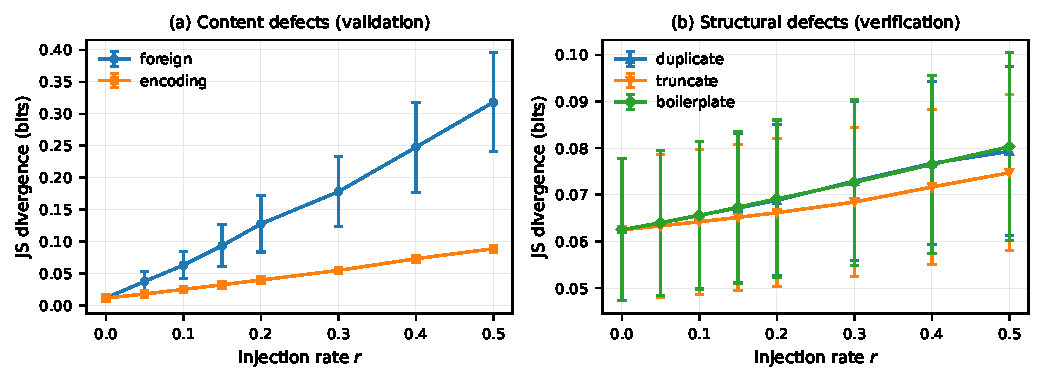
\includegraphics[width=\columnwidth]{fig_dose_response.pdf}
\caption{Dose--response under RGT. (a) Content defects produce steep,
well-separated responses. (b) Structural defects produce only a shallow rise,
as Section~\ref{sec:framework} predicts. Error bars are one standard deviation,
$n=60$.}
\label{fig:dose}
\end{figure}

\subsection{The frequency profile fails on encoding corruption}
Table~\ref{tab:sig} compares clean ($r{=}0$) against lightly defective
($r{=}0.05$) corpora using a one-sided Mann--Whitney $U$ test \cite{mann1947} and
Cohen's $d$ \cite{cohen1988}.

On foreign-text contamination both instruments detect the defect, the
information-theoretic measure with an effect size approximately six times larger
($d=2.48$ versus $0.42$).

On encoding corruption the frequency profile does not merely underperform; it
inverts. Its mean falls as corruption rises over the first three rate steps, it
is monotonic in only four of seven steps, and its effect size is negative
($d=-0.80$, $p=1.000$): it reports a more heavily corrupted corpus as
\emph{more} similar to its clean reference. RGT detects the same defect at
$p\approx2\times10^{-14}$. Fig.~\ref{fig:baseline} shows the contrast.

The mechanism is instructive. Mojibake substitution replaces high-frequency
characters with rare symbols, flattening the frequency profile toward uniformity.
A mean of absolute frequency differences shrinks as both profiles flatten,
whereas a probability-weighted information measure registers the growing cost of
coding one distribution under the other. Whether a real defect is detected or
actively concealed thus depends on the choice between a frequency heuristic and
an information-theoretic quantity.

\begin{table}[t]
\caption{Clean ($r{=}0$) vs.\ lightly defective ($r{=}0.05$), $n=60$ per group,
corpus-level instrument. One-sided Mann--Whitney $U$; Cohen's $d$. With five
defect classes tested, the Bonferroni-corrected threshold is $\alpha=0.010$.}
\label{tab:sig}
\centering
\small
\setlength{\tabcolsep}{4pt}
\begin{tabular}{@{}lrrrr@{}}
\toprule
& \multicolumn{2}{c}{RGT} & \multicolumn{2}{c}{Frequency profile} \\
\cmidrule(lr){2-3}\cmidrule(lr){4-5}
Defect & $d$ & $p$ & $d$ & $p$ \\
\midrule
foreign     & $+2.48$ & $2.1{\times}10^{-21}$ & $+0.42$ & $0.008$ \\
encoding    & $+1.93$ & $2.0{\times}10^{-14}$ & $-0.80$ & $1.000$ \\
duplicate   & $+0.30$ & $0.047$               & $+0.08$ & $0.155$ \\
boilerplate & $+0.11$ & $0.267$               & $+0.04$ & $0.269$ \\
truncate    & $+0.04$ & $0.393$               & $+0.06$ & $0.207$ \\
\bottomrule
\end{tabular}
\end{table}

\begin{figure}[t]
\centering
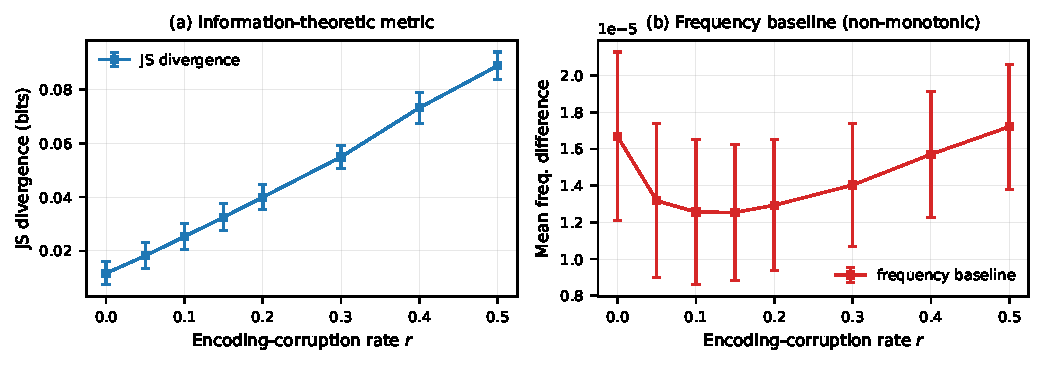
\includegraphics[width=\columnwidth]{fig_baseline_failure.pdf}
\caption{Encoding corruption. (a) The information-theoretic measure rises
monotonically. (b) The frequency profile is non-monotonic, decreasing over the
first three rate steps: it reports increasing corruption as increasing
similarity.}
\label{fig:baseline}
\end{figure}

\subsection{The framework's prediction is confirmed}
Table~\ref{tab:sig} also bears on the prediction of
Section~\ref{sec:framework}. The two content defects are detected with large
effect sizes ($d=2.48$ and $1.93$) and survive Bonferroni correction
comfortably. Of the three structural defects, none survives correction: the
largest, duplication, reaches $p=0.047$ against a corrected threshold of
$0.010$, and its effect size of $0.30$ is $6.5$ times smaller than the weaker of
the two content effects. Corpus-level divergence therefore separates the two
defect categories sharply, as predicted, even though duplication is not entirely
invisible to it.

Moved to the document level, the same structural defects are detected without
error (Table~\ref{tab:doclevel}): ROC-AUC of $1.000\pm0.000$ at every injection
rate tested, over 60 runs each. The verification/validation distinction thus
makes a correct, falsifiable prediction about which instrument succeeds,
converting a descriptive taxonomy into an operational one.

\begin{table}[t]
\caption{Structural defects: corpus-level vs.\ document-level detection.
AUC is mean $\pm$ s.d.\ over 60 runs.}
\label{tab:doclevel}
\centering
\small
\begin{tabular}{@{}lcc@{}}
\toprule
Defect & Corpus-level $d$ ($r{=}.05$) & Document-level ROC-AUC \\
\midrule
truncate  & $0.04$ & $1.000 \pm 0.000$ \\
duplicate & $0.30$ & $1.000 \pm 0.000$ \\
\bottomrule
\end{tabular}
\end{table}

\section{Case Study: Naturally Occurring Defects}
\label{sec:casestudy}

Injected defects are synthetic by construction. During development our own
preprocessing pipeline produced three defects that were not injected, and which
therefore serve as a small sample of naturally occurring faults. Each is a
verification failure in the sense of Section~\ref{sec:framework}, and each was
invisible to aggregate content statistics---the instrument the framework predicts
would miss it.

\textbf{A segmenter that returned a single document.} Segmentation on blank lines
returned the Qur'\={a}n, which is stored one verse per line and contains none, as
a single document of $706{,}471$ characters rather than approximately two
hundred. Foreign-contamination injection was consequently inserting an entire
book rather than a comparable document. The resulting divergence was large
($\approx0.96$ at $r=0.25$) and was an artifact of document size rather than of
language; the value under correct segmentation is $0.088$. Document-length
inspection, the document-level instrument, exposes this immediately.

\textbf{A tokenizer that destroyed the script it measured.} A tokenizer built on
the regular expression \verb|\w+| silently discards Unicode category
\textsf{Mn} (nonspacing combining marks). Applied to the fully vocalized
Qur'\={a}n, every diacritic acted as a word boundary, shattering words into
single letters: $285{,}735$ apparent tokens of only $207$ types, the Arabic
letter inventory. A Unicode-aware pattern,
\verb|[\p{L}\p{N}][\p{L}\p{N}\p{M}]*|, yields $77{,}429$ tokens and $21{,}117$
types. No corpus-level divergence would have revealed this; the type--token
relationship does.

\textbf{Ground-truth labels that penalized a correct detector.} Duplicate
detection initially scored AUC $0.947$ because labels marked only the overwritten
document and not the one it was copied from, penalizing a detector that correctly
flags both members of a pair. With labels corrected, AUC is $1.000$.

These cases support the framework in a setting where the defects were not planted
for the purpose, and they illustrate a practical point: a preprocessing fault can
present as a strong experimental result. The first, in particular, would have
appeared as an exceptionally clear detection had it gone unexamined.

\section{Threats to Validity}

Our substrate is literary and scriptural public-domain text rather than the
newswire and web corpora that motivate the work; absolute divergence values will
differ on other genres. We therefore avoid absolute interpretive thresholds and
rely on the within-corpus null distribution the injection protocol supplies.

Injected defects are synthetic. They are drawn from the classes reported in real
audits \cite{kreutzer2022,dodge2021}, and Section~\ref{sec:casestudy} adds a
small number of naturally occurring cases, but real corpora may exhibit
correlated or subtler defects. Synthetic injection buys a known answer at the
cost of realism; we consider this the correct trade for establishing detection,
and a precondition for studies on naturally occurring defects.

RGT trades formal metricity for adaptivity, as quantified in
Section~\ref{sec:props}. For detection this is immaterial, but applications
requiring the triangle inequality should use fixed smoothing.

Finally, divergence from a reference is not the same as poor quality: a corpus in
a new genre \emph{should} diverge from an established reference. Our protocol
sidesteps this by comparing a corpus against a clean sample of itself, which we
recommend as general practice.

\section{Conclusion}

We have treated corpus verification and validation as an engineering process with
measurable outcomes, and supplied three components: a framework that maps defect
classes to detection instruments, a parameter-free divergence estimator, and a
controlled ground truth against which detection can be demonstrated rather than
illustrated.

Reciprocal Good--Turing smoothing removes a free parameter whose choice we showed
can alter measured effect size threefold, self-adapts across n-gram orders by two
orders of magnitude, and produces conservative estimates with larger effect sizes
than any fixed $k$ examined on the harder content defect. The measure is
monotonic in defect rate for all five defect classes, whereas a frequency-profile
baseline is non-monotonic on encoding corruption and reports it with the wrong
sign. Finally, the verification/validation distinction correctly predicts which
instrument detects which defect: content defects at the corpus level with effect
sizes at least $6.5\times$ those of structural defects, and structural defects at
the document level with ROC-AUC $=1.000$.

Future work should extend the injection protocol to parallel corpora, where a
misalignment injector permits the same treatment of sentence- and
paragraph-alignment pipelines, and should evaluate the estimator against corpora
carrying naturally occurring, human-annotated defects.

\section*{Reproducibility}
All corpora are public domain; the estimator, injection harness, experiment
drivers, and analysis scripts are released with fixed random seeds, and every
figure and table regenerates from them.

\bibliographystyle{IEEEtran}
\bibliography{refs}

\end{document}